%%chapter7

% !TeX spellcheck = en_GB

%\blankpage
%\blankpage
\chapter{MultiView--Ring Calibration}\label{chap:chapter6}
{	\onehalfspacing
	\vspace{4cm}	
	
	The lack of well--characterised VLBI calibrators in the Southern Hemisphere limits the number of targets available within a given radius of a target. This is especially detrimental when conducting astrometry within the Galactic Plane where there is additional obscuration and many radio continuum surveys stop as they approach the plane (usually $|b|\le5$~deg). For traditional phase referencing, this means observations have to rely on `distant' and/or poor quality quasars, or luck. The only alternative to these three is not to conduct observations at all. This is extremely unfortunate as the vast majority of the central Galaxy is visible from the Southern Hemisphere.
	
	The standard approach for phase referencing observations is to seek calibrators as close as possible to the target so as to minimise the differential effects of uncompensated delays. However, as I have shown in the previous chapter, phase referencing using more distant quasars should be possible if the differential delay effects can be measured and hence corrected for.
	
	In this chapter I present results of the first demonstration of inverse MultiView, the first phase referencing observations utilising the ASCI Array and first microarcsecond astrometric result in the Southern Hemisphere. I provide an overview of the processes I personally undertook to achieve this, including scheduling, observing, correlating, reduction and analysis. I then discuss results, uncertainty limitations of the technique and recommendations for future observations.

}
	\singlespacing

\newpage
\section{Introduction}
	The primary cause of residual delay at mid--frequencies ($\sim4-8$~GHz) is generally attributed to the ionosphere. While this is most likely accurate, it does not eliminate the existence of other unmodelled residual delays such as baseline errors or residual troposphere and they should not be discounted. Regardless, due to the much lower density of GPS receivers in the Southern Hemisphere relative to the North, Total Electron Content (TEC) maps have a much lower resolution and can include systematic offsets \citep{WalkerChatterjee1999}. At centimetre wavelengths (e.g. 6.7 or 8.4~GHz) the contribution of tropospheric and ionospheric path delays is expected to be roughly equal, and without a method to remove dispersive and non-dispersive delays separately the residual dispersive delays are included in the solution of the zenith non-dispersive delays. While dual--frequency observations allow accurate tropospheric delays to be measured and applied to phase reference data, residual ionospheric delays will still be present and unmodelled. Therefore, this issue of unmodelled residual delays is shared between dual and single--frequency phase referencing observations and requires observational techniques to remove.
	
	Only derivations of MultiView provide a method to calibrate out these residual ionospheric delays for phase referencing astrometry. These experiments provide the opportunity to not only develop and test these techniques, but to do so on a fledgling VLBI array. The array used for these observations is the AuScope--Ceduna Interferometer (ASCI) Array (\hyperref[sec:spirals]{Section~\ref*{sec:spirals}}). This array will also form the basis for the \spirals\space large project, and these observations serve as pilots in terms of array capabilities and technique. 
	
	The AuScope portion of this array is comprised of Katherine (Ke), Yarragadee (Yg) and Hobart26m (Ho). Ke/Yg are identical $12$\,m Patriot geodetic dishes equipped with S/X receivers, DBBC2 digitisers and Mark5B recording units \citep{Lovell2013}. Ho is a 26m X/Y mount equipped with cryogenic cooled L, S, X, C(4.8~GHz), 6.7~GHz, 12~GHz, S/X and K--band receivers, DBBC2 and Fila10G/Flexbuf recorder. Ho/Ke and Yg all regularly participate in IVS geodetic observations. The final telescope, Ceduna \citep[Cd; ][]{McCulloch2005} only participates in irregular LBA VLBI observations. It is a 30\,m ex-telecommunications dish, equipped with uncooled L, S, X, C(4.8~GHz), 6.7~GHz, 12~GHz and K--band receivers, a DBBC2 and Fila10G/Mark5C recorder. This will be the first time these telescopes will be used in conjunction for VLBI astrometry and I am eager to show how they perform.

	\spirals\space aims to achieve high accuracy astrometry for 6.7~GHz masers on the ASCI array, however, it will likely encounter the same large residual delays as \citet{Krishnan2015,Krishnan2017} on the LBA. Authors of those papers suspect the main cause of residual delay was the ionosphere and therefore MultiView may be the only way to remove those effects. In fact, as I have shown in \hyperref[chap:chapter5]{Chapter~\ref*{chap:chapter5}} MultiView should be able to calibrate almost all causes of residual delay. Therefore I want to collect and analyse real data to test these predictions.

	In this chapter I develop the methodology and reduction processes for inverse MultiView, allowing for high accuracy astrometry at intermediate frequencies in the presence of suspected large residual delays. The questions that I address are:
	\begin{enumerate}
		\item What is the astrometric accuracy of MultiView vs. what would be expected from inverse phase referencing at a similar target--calibrator separation. Does it perform better? As I will show, inverse MultiView increases calibration overheads and is non trivial to observe or reduce. Does it return a proportionally better result? I address this question in \hyperref[sec:mvastrometry]{Section~\S\ref*{sec:mvastrometry}};
		\item What is the maximum separation between target and calibrators for which inverse MultiView can measure coherent solutions and what is the cause of this decoherence? There are generally fewer suitable (compact, high flux density) calibrators in the immediate neighbourhood of Galactic masers so the larger separation for which high accuracy astrometry can be undertaken, the better. \citet{Rioja2017} use a maximum separation between calibrators of $\theta\sim10$~deg at low frequencies for non--inverse MultiView, where the ionosphere is expected to be the largest source of error. At higher frequencies ($>6-8$~GHz) the troposphere is expected to be dominant, however, the residual effects of both can be equivalent in magnitude. So after including dry tropospheric calibration techniques (geoblocks) and GPS TEC maps, is MultiView at intermediate frequencies limited by ionosphere, dry/wet troposphere or some other factor? I address this question in \hyperref[sec:mvastrometry]{Section~\S\ref*{sec:mvastrometry}}.
		
		\item Is it possible to use measured phase slopes to determine residual delays? The derived equations in the \hyperref[chap:chapter5]{previous chapter} provide clear relationships between instantaneous sources of residual delay, LST and/or UTC, longitude, latitude, RA and DEC. It is possible to de--couple the relationships and approximate residual path delay and therefore estimate the calibration fidelity. The phase--slopes derived in the previous chapter are very sensitive to residual delay and therefore could be used as a delay probe. I discuss the nature of phase slopes and feasibility of delay determination in \hyperref[sec:phaseslopes]{Section~\S\ref*{sec:phaseslopes}}.	
			
		%\item Following on from the previous question: Is there a clear time--scale for variability in the measured phase slopes indicative of the various sources of delay aka. baseline error vs. troposphere? If the sources of delay can be de--coupled then the various unknown time scales might be able to be determined. The residual ionospheric and wet--tropospheric time scales are theoretically uncertain (\hyperref[chap:chapter5]{see chapter 5}) and approximate determination via this technique might be possible.  I address this question in \hyperref[]{Section \S~\ref*{}}.
		\item How should MultiView be conducted in the future? Is there an optimal number of calibrators, what calibrator parameters should be optimised and what spacing/positioning might give best results.  I address this question in \hyperref[sec:astrouncertainty]{Section~\S\ref*{sec:astrouncertainty}}.
	\end{enumerate} %{\R why are these questions important}

\section{Source Selection}
    The ultimate aim of this chapter is to test the ability of inverse MultiView to measure and remove the residual delay for maser astrometry in \spirals, so the observing structure is nearly identical to that of a maser phase--referencing observation (see \hyperref[sec:obsstruct]{Section~\S\ref*{sec:obsstruct}}). The ASCI array does not currently have mutual frequency coverage over the rest frequencies of any known and/or appropriately bright maser species, so I have used quasars as both the calibrators and targets for these MultiView tests. Although this does not allow me to test MultiView under identical conditions as a parallax observation, it does present other advantages. In the next few sections I will discuss these advantages and quasar selection criteria.
    
    \subsection{Quasar benefits and Quality $\boldsymbol{Q}$}
    	The primary benefit of using quasars as targets is that their positions are constant with time. In addition, they have little to no structure and due to frequent observations by global VLBI arrays, often have known positional and flux density values. The lack of detectable proper motion and parallax implies any measured offsets that change over time are due to residual delay or phase--noise, which can be directly used for an estimate of calibration quality. This fact will be used to compare traditional phase referencing methods to inverse MultiView and determine the overall capability of the array.
    	
    	Although many quasars can appear point--like, others can have jets that may offset the astrometric results. Care is taken to avoid resolved quasars or those with jets as they can make phase referencing solutions confusing or add positional uncertainty. Frequent VLBI observations of a subset of quasars places good constraints on their absolute positions. Henceforth I will refer to the positional uncertainty of a quasar as its quality $Q$. Generally speaking, the smaller $Q$ is, the more desirable the quasar is for astrometry
    	
    	Another advantageous characteristic of quasars is that they are very common compared to masers (referring to individual maser regions per species). The 2019a Radio Fundamental Catalogue contains 15740 objects\footnote{http://astrogeo.org/rfc/}, which gives an average sky density of $\sim0.38$\,deg$^{-2}$ or roughly 1.2 quasars per circle of radius 1\,deg. In contrast, the catalogue of all known 6.7\,GHz methanol masers \citep[][ and referenced therin]{Yang2019} contains 1085 masers largely confined to the Galactic Plane $|b|<5^\circ$ and only observable between $7-17$ LST for the Southern Hemisphere. This difference not only allows for a larger pool to select from and a greater time window to observe, but allows one to have strict selection criteria. 
    	
    	While the total quasar sky--density remains $0.38$\,deg$^{-2}$ at intermediate--to--high Declinations, at low Declinations ($\delta < -30^{\circ}$) the total density drops to $\sim0.19$\,deg$^{-2}$ (\hyperref[quasarrainbow_hist]{Figure~\ref*{quasarrainbow_hist}}). This discrepancy is unlikely due to a lack of quasars, which are isotropically distributed but represents a relatively lower amount of regular and high--sensitivity quasar surveys in the Southern Hemisphere. In addition, due to the relative lack of frequent observations, the number of quasars known in the Southern Hemisphere is proportionally biased towards `low--quality' quasars (\hyperref[quasarrainbow_hist]{Figure~\ref*{quasarrainbow_hist}}).
    	\begin{figure}[h]
    		\centering
    		\includegraphics[width=.75\textwidth]{quasar_hist.pdf} 
    		\caption[Quasar Quality Histogram]{Stacked Declination--binned quasar density distribution. Colour represents relative contribution of each quasar-$Q$ (legend) to the Declination--binned quasar density.}
    		\label{quasarrainbow_hist}
    	\end{figure}
    	In catalogues, quasars are presented with estimated positional accuracies. As I want to focus on the atmospheric aspects of MultiView calibration, I chose only quasars with $Q<0.3$~mas.  Finally, to limit the effects of target elevation, sources are only selected from the South celestial region $\delta<0$. Next, I need to consider quasars from the perspective of array sensitivity. 
	    %Positional inaccuracy is a limiting factor for even MultiView and therefore should be minimised as much as possible, $Q=0.3$~mas corresponds to the 
    %\clearpage
    \subsection{Sensitivity Limitations}   			
    	I want to use the nominal SEFDs of the telescopes to determine the detection limit. Taking the Cd--Ke baseline and nominal $\text{SEFD}=800$~Jy and $\text{SEFD}=3500$~Jy for Ceduna and Katherine respectively, a $\tau=40$~s integration with a spanned-bandwidth of $\Delta\nu=256$~MHz will yield a noise level $\sigma_S$ of: 	
    	\begin{align*}
    		\sigma_N & = 1.2\sqrt{\frac{\text{SEFD}_i~\text{SEFD}_j}{2\tau\Delta\nu}}=1.2\sqrt{\frac{800\times3500}{2\times40\times256\times10^{6}}} \\
    		& = 11\text{\,mJy}
    	\end{align*}    	
    	Therefore, for a strong, per-scan detection of $\text{SNR}=\frac{S_c}{\sigma_N}>10$, I require quasars with a correlated flux density $S_c>110\text{\,mJy}$. Constraining $S_c$, $\delta<0.0$~deg and $Q<0.3$~mas I find there are a total of 824 available quasars. From this list of good quasars, I desire the ones which have a sky distribution favourable for testing inverse MultiView.
    	\begin{figure}[h]
    		%\centering
    		\includegraphics[width=.75\textwidth]{quasar_good.pdf} 
    		\caption[Good quasars]{Sky positions of all $\delta<0.0^{\circ}$ quasars. {\bf Black:} Non--suitable quasars due to positional uncertainty $Q>0.3$\,mas. {\bf Blue:} Non--suitable quasars on the basis of catalogued correlated flux $S_c<110$\,mJy. {\bf Red:} All suitable quasars.}
    		\label{quasarpos_good}
    	\end{figure}
       
    \subsection{Quasar Arrangement}
		The final determination is to choose which clusters of quasars I want to select as the targets and calibrators from this list of 824 quasars. The expectation is that for a clumpy and non--uniform residual ionosphere, there should be a maximum distance beyond which phase decoherence occurs. In order to test this theory I use the idea of a calibration ring with an approximate radius around a target quasar to compare the astrometric accuracy for each ring radii. 
		
		A search was conducted for quasars that had $N\ge6$ surrounding quasars within the sample, confined to ring radii or range 2--4, 4--5, 5--6, 6--7 and 7--8 degrees. The number of quasars in the ring was chosen for redundancy and in order to minimise the contribution from directionality. Quasar clusters were selected from the sample that had good position angle ($\theta_i=\arctan (\Delta\delta,\Delta\alpha)$) sampling about the target such that the root sum of squares (RSS) of the angle was:
		\begin{equation*}
			\text{RSS} = \frac{\sqrt{\sum\theta_i^2}}{2\pi} \le 1.2
		\end{equation*} In total this gave a list of 29 potential rings. Visual inspection of the rings was performed to cut down list of candidates to 9. Three at around $\alpha=7$~hrs, $\alpha=14$\,hrs and $\alpha=20$\,hrs. The three rings would share a 7~hour track over a $\sim24$~hour experiment, sampling the different radii and effects due to Local Time.
		
		Largely for historical and internal reasons, sources names are indicated via the following rules: Source names starting with G indicates a target at the centre of a ring, J indicates a calibrator (orbit source) within the ring and F a fringe finder. In all cases the name of the sources is based on the J2000 right ascension and declination.
		
		Pathfinder observations MV022 and MV025 revealed that some of these rings contained poorly constrained calibrator and target positions and/or lower flux density sources than expected from the catalogued values. Therefore the final list of rings was cut down to the best 3 at differing LST and radii in experiments MV026, 27 and 28. These rings were centred at the quasar positions of: G0634--2335 with a mean radius of $\overline{R}=3$~deg; G1901--0809 with $\overline{R}=6.5$~deg and; G1336--0829 with $\overline{R}=7.5$~deg (see \hyperref[j0634ring]{Figures~\ref*{j0634ring}},~\ref{j1336ring} and~\ref{j1901ring}, respectively). Considering the isoplatonic radius for the wet--troposphere is considered to be smaller than $R=7-9$~deg, this was expected to give a good idea of the limitations of inverse MultiView calibration before and after this transitional point.
		
		\begin{figure}[h]
			\centering
			\includegraphics[width=0.75\textwidth]{G0634-2335.pdf} 
			\caption[G0634-2335 Ring Plot]{Ring plot for target quasar G0634--2335. This ring is between $2^\circ$ and $4^\circ$ as smaller rings with sufficient quasars that fit the criteria did not exist. The catalogued correlated flux density for G0634--2335 is 467\,mJy.}
			\label{j0634ring}
		\end{figure}
		
		\begin{figure}[h]
			\centering
			\includegraphics[width=0.75\textwidth]{G1336-0829.pdf} 
			\caption[G1336-0829 Ring Plot]{Ring plot for target quasar G1336--0829. This ring is between $7^\circ$ and $8^\circ$ and the central quasar has flux density 219\,mJy.}
			\label{j1336ring}
		\end{figure}
		
		\begin{figure}[h]
			\centering
			\includegraphics[width=0.75\textwidth]{G1901-2112.pdf} 
			\caption[G1901-2121 Ring Plot]{Ring plot for target quasar G1901--2112. This ring is between $6^\circ$ and $7^\circ$ and the central quasar has flux density 120\,mJy.}
			\label{j1901ring}
		\end{figure}
		
    
\clearpage	
\section{Method and Observations}
	\subsection{Array and Frequency}
		Observations were conducted using the ASCI Array (\hyperref[sec:spirals]{Section \S\ref*{sec:spirals}}). Baselines and approximate sensitivities are given in \hyperref[tab:ascibaselines]{Table~\ref*{tab:ascibaselines}}. The ASCI Array is quite sparse, lacking baselines $uv<45$~M$\lambda$. For compact targets and calibrators such as those determined in \hyperref[chap:chapter4]{Chapter \S\ref*{chap:chapter4}} or chosen in the previous section, this sparse $uv$--sampling should prove less of an issue, with the exception of potentially higher sidelobe levels than an array with more elements.
		\begin{table}[H]
			\centering
			\caption[ACSI baselines]{{\bf Left:} VLBI baselines for the ASCI Array. {\bf Upper Left:} Linear distances (km) between the antennas as calculated by NRAO VLBI scheduling program SCHED. {\bf Lower Left:} Approximate mean $uv$-distance (M$\lambda$) for 8.34\,GHz  observations. {\bf Right:} Baseline sensitivites ($\pm10\%$, mJy) for a 40~s integration and $\Delta\nu=256$~MHz. }\label{tab:ascibaselines}
			{\onehalfspacing\small
				\begin{tabular}{l| rrrr |rrrr}
					\toprule
		            \hline
				            &        &$|\textbf{B}|$&  &        &&$\boldsymbol{\sigma_S}$&\textbf{(Jy)}&           \\\hline
						    &{\bf Cd}&{\bf Ho}&{\bf Ke}&{\bf Yg}&{\bf Cd}&{\bf Ho}&{\bf Ke}&{\bf Yg}\\ \hline
					{\bf Cd}&  -     & 1703   & 1937   & 1792   & -      &        &        &        \\
					{\bf Ho}& 47.3   &   -    & 3432   & 3211   & 5      & -      &        &        \\
					{\bf Ke}& 53.9   &  95.4  &  -     & 2360   & 11     & 9      & -      &        \\
					{\bf Yg}& 49.8   &  89.3  & 65.6   &   -    & 11     & 9      & 21     &  -     \\\bottomrule
				\end{tabular}
			}
		\end{table}
		The optimal frequency range to observe the quasars was deemed to be X--band due to mutual frequency coverage, ionospheric/tropospheric stability and most importantly, frequency--proximity to the planned observing frequency of 6.7~GHz methanol masers. S--band was also an available option for mutual frequency coverage, but lacked other factors. If the aims had been to test ionospheric residual delay and compensation by MultiView, perhaps future observations could involve this. However, in order to test inverse MultiView as applicable to maser phase referencing, X--band was the best option.
		
		All observations were recorded with 16\times16~MHz packed bands, single polarisation RCP, giving 256~MHz sky frequency and the following setup:
		\begin{equation*}
		\nu_L = 8196.99+16\times(0,1,2,3,4,5,6,7,8,9,10,11,12,13,14,15)~\text{MHz}
		\end{equation*} where $\nu_L$ is the lower edge frequency for each band. Single polarisation 256~MHz was chosen over the optional 128~MHz dual polarisation as the former prioritises delay sensitivity and the latter discrete frequency sensitivity. As quasars emit in continuum, wide--band single polarisation was prioritised.
	    	
	\subsection{Observing Structure} \label{sec:obsstruct}
		The general observing structure is modelled on that used for the VLBA BeSSeL BR210 epochs (see \hyperref[sec:standardvlbicalibration]{Section~\S\ref*{sec:standardvlbicalibration}} and \hyperref[chap:chapter3]{Chapter~\ref*{chap:chapter3}}) and consists of three full tracks spanning $\sim23$~hours. Each 7~hour track is defined as the time in which the target source is at an elevation above $30^{\circ}$ at all stations, bracketed by $45$~mins for calibration (see \hyperref[fig:mvobservingblockdiagram]{Figure~\ref*{fig:mvobservingblockdiagram}}).
		
\tikzstyle{line}   = [draw,-stealth,thick]
\tikzstyle{block}  = [draw,rectangle,text width=17em,minimum height=10mm, node distance=3em]
\tikzstyle{gblock} = [draw,rectangle,text width=17em,minimum height=10mm, node distance=3em,fill=green!10]
\tikzstyle{fblock} = [draw,rectangle,text width=17em,minimum height=10mm, node distance=3em,fill=yellow!10]
\tikzstyle{eblock} = [draw,rectangle,text width=17em,minimum height=5mm, node distance=3em,fill=black!10]
\tikzstyle{nblock} = [draw,rectangle,text width=17em,minimum height=5mm, node distance=3em]

\tikzstyle{bwbloc} = [draw,rectangle,text width=17em,minimum height=60mm,node distance=2em]
\tikzstyle{tblock} = [draw,rectangle,text width=10em,minimum height=6mm, node distance=2em,fill=blue!10]
\tikzstyle{cblock} = [draw,rectangle,text width=10em,minimum height=6mm, node distance=2em,fill=red!10]
\tikzstyle{wblock} = [draw,rectangle,text width=10em,minimum height=6mm, node distance=2em]

		\begin{figure*}
			\vspace{2em}
			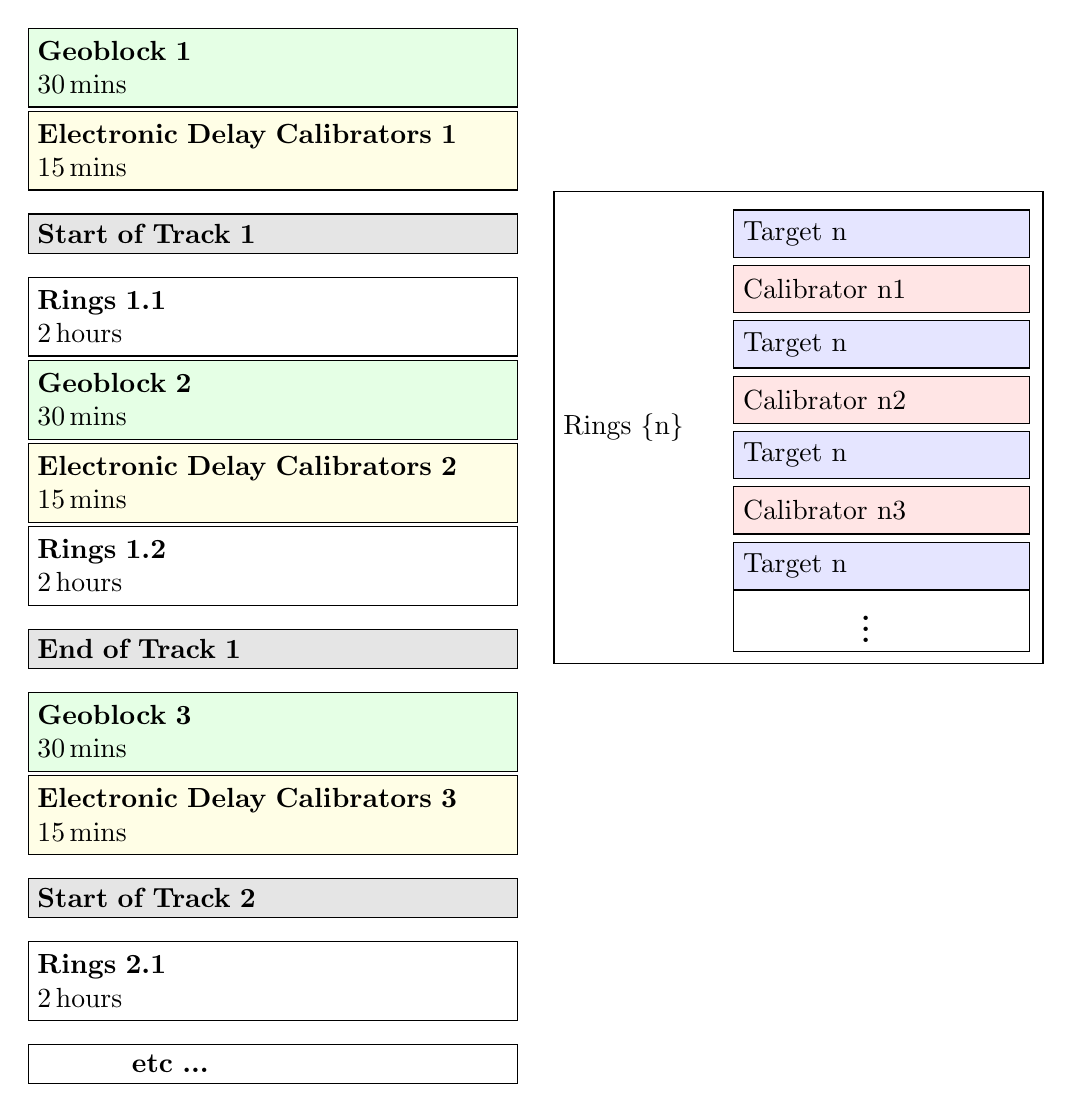
\begin{tikzpicture}
			\node [gblock](start2){ {\bf Geoblock 1}\\ 30\,mins};
			\node [fblock,below of=start2](proc 1){ {\bf Electronic Delay Calibrators 1}\\ 15\,mins};
			\node [eblock,below of=proc 1](start1){\bf Start of Track 1};
			\node [ block,below of=start1](proc 4){ {\bf  Rings 1.1}\\2\,hours};
			
			\node [gblock,below of=proc 4](proc 5){ {\bf  Geoblock 2}\\ 30\,mins};
			\node [fblock,below of=proc 5](proc 6){ {\bf  Electronic Delay Calibrators 2}\\ 15\,mins};
			\node [ block,below of=proc 6](proc 9){ {\bf Rings 1.2}\\2\,hours};
			\node [eblock,below of=proc 9](proc 14){\bf End of Track 1};
			\node [gblock,below of=proc 14](proc 10){ {\bf Geoblock 3}\\ 30\,mins};
			\node [fblock,below of=proc 10](proc 11){{\bf  Electronic Delay Calibrators 3}\\ 15\,mins};
			
			\node [eblock,below of=proc 11](start12){\bf Start of Track 2};
			\node [ block,below of=start12](ring22){ {\bf  Rings 2.1}\\2\,hours};
			\node [nblock,below of=ring22](end){\hspace{1.2cm}{\bf etc ...}};
			
			\node [bwbloc,right of=proc 4,xshift=17em,yshift=-4em](explain){Rings \{n\} };
			\node [tblock,right of=start1,xshift=20em](explain 1){Target n};
			\node [cblock,below of=explain 1](explain 2){Calibrator n1};
			\node [tblock,below of=explain 2](explain 3){Target n};
			\node [cblock,below of=explain 3](explain 4){Calibrator n2};
			\node [tblock,below of=explain 4](explain 5){Target n};
			\node [cblock,below of=explain 5](explain 6){Calibrator n3};
			\node [tblock,below of=explain 6](explain 7){Target n};
			\node [wblock,below of=explain 7](explain 8){\hspace{1.5cm}{\bf \vdots}};
			\end{tikzpicture}
			\caption{Block Diagram for the MV02* observing structure.}
			\label{fig:mvobservingblockdiagram}
			\vspace{2em}
		\end{figure*}
		Observations begin with a 30~minute geoblock, followed by a $\sim$15~min block with electronic delay calibrators (EDC). For redundancy, 3--4 bright fringe finder quasars sources were scheduled in each EDC to ensure that one or more is sufficiently bright and has enough onsource time. Slewing accounts for the remaining time. Potentially overzealous redundancy was due to uncertain quasar brightness and array performance. The fringe finders were used to calculate clock drift--rate, bulk clock--offsets and confirm fringes during correlation, calibrate individual telescope electronic delays (manual phase calibration) as well as check delay residuals after application of global atmospheric delay solution. Although the pre--calibration (geoblock + fringe finder) overhead is about 30\%, good {\it a priori} solutions for the delays and fringe--rates are required to avoid the possibility of phase--wrap ambiguities. As seen in the previous chapter, the magnitude of the delay/phase planes depends on residual delay and might cause general loss of coherence in the phase domain if left uncalibrated.
		
		At beginning of the track after the first geoblock and EDC block, the target source was at an elevation $\varepsilon\gtrsim30^{\circ}$ at all sites and the MultiView nodding began. The observing mode here was Target, Calibrator 1, Target, Calibrator 2, ... and so on. For eventual fringe--fitting on the target (inverse phase referencing), target source scans observations bracket the calibrator scans to ensure long--term phase coherence. I decided it was best to observe orbit sources in a `star' pattern rather than progressing azimuthally around the ring. This was to minimise the effect of a possible directional sampling bias and ensuring that the slope measured at any time was representative. There may be more a optimal time--spatial sampling for a given quasar distribution that accounts for likely slope differential changes over the loop interval, however, that investigation is a refinement on the basic method and is a potential topic for future study.
				
		The above process was repeated once, with a second geoblock in the centre of the track to avoid loosing time due to tracking the target source through the zenith at the larger, more slowly slewing antennas. The third geoblock and electronic delay calibrator blocks are directly after the target was below $30^{\circ}$ at at least two stations. Geoblocks must also bracket ring blocks for interpolation of clock and tropospheric delay solutions, with a minimum of 3 geoblocks necessary for a reasonable estimate for the clock--rate and residuals at each station. Tracks can be tiled together, sharing the middle and fringe--finder blocks such that observations can contain at least 3 tracks per day for a total of approximately 23~hrs. 

	    \begin{table}[h]
	    	\footnotesize
	    	\centering
	    	\caption[MV observational epochs]{MV02* epochs. \textbf{Top:} Successful epochs, characterised by minimal or acceptable issues and or loss of data. \textbf{Bottom:} Unsuccessful MV02$X$ epochs where one or more major telescope, backend or data problems caused the loss of almost all the data at one or more antennas. }
	    	{\onehalfspacing
	    		\begin{tabular}{lrll} \hline
	    \multicolumn{1}{c}{\bf Epoch} & \multicolumn{1}{c}{\bf Date} & \multicolumn{1}{c}{\bf $N_{r}$} & \multicolumn{1}{c}{\bf Notes} \\ 		
	    \hline
	    {\bf Used:} &&& \\
	    MV025  & 17-Feb-2019 & 9    &  9 ring experiment, otherwise no issues   \\\hline
	    MV026  & 17-Mar-2019 & 3    &  Ceduna~30m power failure in last 3 hours and subsequent clock jump  \\
	    MV027  & 13-Apr-2019 & 3    &  No issues to note  \\
	    MV028  &  4-May-2019 & 3    &  No issues to note  \\\hline
	    \hline
	    {\bf Unused:} &&& \\
	    MV022  &  9-Feb-2019 & 9    &  Unexplained $> 2\,ns$ clock oscillation at Ceduna~30m \\
	    {\bf Unsuccessful:} &&& \\
	    MV020  & 20-Jul-2018 & 9    &  6\,hour pilot observation. No Hobart~26m fringes \\
	    MV021  & 23-Sep-2018 & 9    &  Incorrect Hobart26m mode and bitmask \\
	    MV023  &  9-Feb-2019 & 9    &  Incorrect receiver configuration at Ceduna~30m \\
	    MV024  & 10-Feb-2019 & 9    &  Incorrect Mark5B frame size at Ceduna~30m, data recorded incorrectly; \\ &&& Katherine taken offline after 6\,hours for maser maintenance \\
	    \hline
	    		\end{tabular}
	    	}
	    \label{tab:multiviewepochs}
    	\end{table}
		\hyperref[tab:multiviewepochs]{Table~\ref*{tab:multiviewepochs}} summaries the results of epochs MV020 through to MV028. Only epochs MV025 through to MV028 are used in further analysis for the reasons outlined in the bottom section of \hyperref[tab:multiviewepochs]{Table~\ref*{tab:multiviewepochs}}.

\clearpage
\section{Reduction Processes}	
	The data were all reduced in an identical manner over the four epochs (MV025, 26, 27 and 28) with the Standard VLBI calibration method (\hyperref[sec:standardvlbicalibration]{Section~\ref*{sec:standardvlbicalibration}}) with minor variation:\begin{enumerate}
		\item Some antenna positions needed to be corrected and updated. This was performed by fitting the residual multiband delays for a diurnal sinusoidal offset in addition to geodetic delays;
		\item The amplitudes were initially calibrated with antenna system temperature measurements from the telescope sites, and then again using an iterative method (see \hyperref[sec:altquascal]{Section~\S\ref*{sec:altquascal}});
		\item After manual phase calibration, data is fit with inverse phase referencing (iPR) and can proceed to be split out and imaged. Then, post--iPR  data is fit with inverse MultiView methods and this data is also split out and imaged.
	\end{enumerate}

	\subsection{Correlation}
		I correlated the baseband data from the telescopes with DiFX-2.6.1 \citep{Deller2011} running on a local cluster. As per \hyperref[sec:correlation]{Section~\ref*{sec:correlation}} this process involved fringe verification and manual clock--searching. For fringe--finding, a strong source from the EDC blocks (optimally near the centre of the observation; EDC block 2 or 3) with all telescopes onsource is correlated at a high spectral resolution (often $\delta\nu<0.0625$MHz/channel, or 256 channels in a 16\,MHz band). The detection of fringes on this source indicates that telescopes had a correct frequency setup and indeed was on source for this time (potentially eliminating extreme pointing issues). In addition, high spectral resolution correlation allows the detection of higher single band delays which might otherwise wrap over a channel. The maximum detectable delay goes as $\tau=2\pi/\delta\nu<100~\mu$s, so failure to find fringes might indicate a too low correlation resolution such that the phases are decorrelating over the channels. Once fringes are found, the antenna delays for that scan can be used to zero the delays (within measurement uncertainty of the delay determination). Once clocks were zeroed about the middle of the experiment, all fringe--finder scans were correlated and clocks rates were fit with least--squares regression (\hyperref[fig:correlation]{Figure~\ref*{fig:correlation}}).
	    \begin{figure}[h]
	    	\centering
	    	\begin{subfigure}[t]{0.45\textwidth}
	    		\includegraphics[width=0.9\textwidth]{0.pdf}
	    	\end{subfigure}
	    	~
	    	\begin{subfigure}[t]{0.45\textwidth}
	    		\includegraphics[width=0.9\textwidth]{0res.pdf}
	    		%\caption[Bayesian clock--fitting residuals]{Delays measured on fringe--finder targets Ho--Cd}
	    	\end{subfigure}
	    	\caption[Bayesian clock--fitting]{Delays measured on fringe--finder quasars for experiment MV028, baseline Ho--Cd. \textbf{Left:} fitting and removing clock drift rate between stations. Measured and removed clock rate is $\frac{d\tau}{dt}=97\pm13$~ps/s in this case. The fit for residual electronic delay $\tau_e=1\pm30$~ns. \textbf{Right:} Residual delay after clock removal is $|\delta\tau|<3$~ns which can be explained by individual IF electronic delays or atmospheric effects. This will be removed in \aips\space calibration. The low residual delay allows for a much coarser correlation resolution in FITS output at 0.5~MHz/chan as this will still allow this small delay to be easily detected and corrected during processing.} \label{fig:correlation}
	    \end{figure}	    
	    %The positional uncertainty of Ceduna~30m was believed to be much higher than the other three stations as it only rarely participated in IVS--style VLBI sessions. Those that it did participate in were X--band LBA observations culminating in publishd position in \citep{Leonard2018} aka. AstroGeo. All telescope positions were made consistent with those catalogued at AstroGeo and using X,Y,Z drift rates.s
		Fitted clock--rates were applied and final correlation was performed in one pass - all sources correlated over the full bandwidth (16~MHz) with 32 spectral channels per IF, giving a spectral resolution of 0.5\,MHz.
	    	    
	    %\clearpage

		\subsection{Antenna Position Corrections}
			For correlation I used antenna positions and velocities determined from the information on the AstroGeo website\footnote{http://astrogeo.org/vlbi/solutions/} given in \hyperref[antennapositions]{Table~\ref*{antennapositions}}. These positions come from past IVS and geodesy-style experiments nominally involving the 4 stations of interest as part of the LBA. Hobart~26m, Katherine~12m and Yarragadee~12m partake in IVS experiments at least once per week, and therefore their positions are known to the level of $|\Delta B|\sim1$~cm. Ceduna~30m does not regularly partake in IVS--style experiments and therefore has a more uncertain position.
			\begin{table}[h]
				\footnotesize
				\centering
				\caption[MV02* antenna positions and velocities]{Correlated antenna positions and velocities at epoch 2000.0 from AstroGeo RFC\_2018. Ceduna velocity taken from  RFC\_2009. \textbf{Columns (1)} Antenna name; \textbf{(2-3)} $X$ position and velocity; \textbf{(4-5)} $Y$ position and velocity; \textbf{(6-7)} $Z$ position and velocity.}
				{\onehalfspacing
					\begin{tabular}{lrrrrrr} \hline
						\multicolumn{1}{c}{\bf Antenna} & \multicolumn{1}{c}{$\boldsymbol{X}$} & \multicolumn{1}{c}{$\boldsymbol{\dot X}$} & \multicolumn{1}{c}{$\boldsymbol{Y}$} & \multicolumn{1}{c}{$\boldsymbol{\dot Y}$} & \multicolumn{1}{c}{$\boldsymbol{Z}$} & \multicolumn{1}{c}{$\boldsymbol{\dot Z}$} \\ 
						\multicolumn{1}{c}{} & \multicolumn{1}{c}{(m)} & \multicolumn{1}{c}{(m/yr)} & \multicolumn{1}{c}{(m)} & \multicolumn{1}{c}{(m/yr)} & \multicolumn{1}{c}{(m)} & \multicolumn{1}{c}{(m/yr)} \\
						\hline
						Ceduna~30m     & $-3753442.7457$  & $-0.04173$  &  3912709.7530 & 0.00267     &  $-3348067.6095$  & 0.04990  \\
						%               & $-3753443.6830$  & $-0.03995$  &  3912709.8430 & 0.00550     &  $-3348066.6520$  & 0.04546  \\\hline%% ATNF
						Hobart~26m     & $-3950237.5960$  & $-0.03834$  &  2522347.7530 & 0.00849     &  $-4311561.6600$  & 0.03942  \\
						%		       & $-3950237.4030$  & $-0.03901$  &  2522347.6841 & 0.00796     &  $-4311561.8335$  & 0.04110  \\\hline%% ATNF
						Katherine~12m  & $-4147354.8680$  & $-0.03477$  &  4581542.3320 & $-0.01545$  &  $-1573302.9130$  & 0.05427  \\
						%			   & $-4147354.6913$  & $-0.03771$  &  4581542.3772 & $-0.01159$  &  $-1573303.1565$  & 0.05630  \\\hline %% ATNF
						Yarragadee~12m & $-2388896.4240$  & $-0.04673$  &  5043350.0760 & 0.00824     &  $-3078590.5910$  & 0.04838  \\
						%               & $-2388896.1890$  & $-0.04814$  &  5043350.0019 & 0.00960     &  $-3078590.8037$  & 0.05106  \\\hline%% ATNF
						
						\hline
					\end{tabular}}
					\label{antennapositions}
				\end{table}		
				
				Single--frequency geoblock fitting nominally takes measured LoS delay (after manual phase calibration, EOP and TEC corrections; see \hyperref[sec:standardvlbicalibration]{Section \S\ref*{sec:standardvlbicalibration}}) and fits for a likely clock rate and zenith non--dispersive delay. If other delays are present, they will be included in this fitting process and skew the zenith delay estimate (see \hyperref[sec:drytropotheory]{Section \S\ref*{sec:drytropotheory}}). %Not only does this mean that in the presence of other delays, those due to zenith troposphere can be underestimated, but a valid--looking solution can almost always be found and potentially un--noticed. 
				In the presence of suspected baseline errors, I used an alternate programme (written by Mark J. Reid) to simultaneously fit for tropospheric dispersive delay, clock rate and positional offsets in the Ceduna~30m correlated position $\Delta X$, $\Delta Y$, $\Delta Z$. Results of this fitting are shown in \hyperref[tab:ceduna_offset]{Table~\ref*{tab:ceduna_offset}}.
				\begin{table}[h]
					\footnotesize
					\centering
					\caption[Ceduna position offsets]{Measured position offsets and formal uncertainty for Ceduna~30m over the 4 epochs. *The $Y$ component had a necessary sign reversal when applied. Positional accuracy in epoch MV026 is understandably lower due to positional determination from 6 geoblocks rather than 7 (data flagged following clock jump).}
					{\onehalfspacing
						\begin{tabular}{lcccccc} \hline
							\multicolumn{1}{c}{\bf Epoch} & \multicolumn{1}{c}{$\boldsymbol{\Delta X}$} & \multicolumn{1}{c}{$\boldsymbol{\sigma_{\Delta X}}$} & \multicolumn{1}{c}{$\boldsymbol{\Delta Y}$} &\multicolumn{1}{c}{$\boldsymbol{\sigma_{\Delta Y}}$} & \multicolumn{1}{c}{$\boldsymbol{\Delta Z}$} & \multicolumn{1}{c}{$\boldsymbol{\sigma_{\Delta Z}}$} \\
							& \multicolumn{1}{c}{\textbf{(cm)}} & \multicolumn{1}{c}{\textbf{(cm)}} & \multicolumn{1}{c}{\textbf{(cm)}} & \multicolumn{1}{c}{\textbf{(cm)}} & \multicolumn{1}{c}{\textbf{(cm)}} & \multicolumn{1}{c}{\textbf{(cm)}} \\\midrule
							MV025	&	5.31	&	2.67	&	9.24	&	2.66	&	24.23	&	2.31	\\
							MV026	&	8.69	&	2.88	&	10.97	&	2.99	&	21.43	&	2.94	\\
							MV027	&	6.09	&	2.64	&	6.87	&	2.68	&	20.55	&	2.60	\\
							MV028	&	6.83	&	2.67	&	9.13	&	2.72	&	22.87	&	2.62	\\\hline
							\textit{AVG}	&	6.7	&	1.4	&	$-9.1$*	&	1.4	&	22.3	&	1.3	\\
							\bottomrule
						\end{tabular}} \label{tab:ceduna_offset}
					\end{table}	
					
					\begin{SCfigure}[][h]
						\centering
						\includegraphics[width=.55\textwidth]{ceduna_pos.pdf}
						\caption[AstroGeo vs. SCHED Ceduna Position]{Ceduna X (red), Y (blue) and Z (green) position vs. time for SCHED (solid) and AstroGeo (dotted) catalogued positions as compared to the mean position determined at all MV02* epchs (black + error bars).} \label{fig:astrovssched}
					\end{SCfigure}
					
					I measured the Ceduna~30m position offset to be $(\Delta X, \Delta Y, \Delta Z)=(7,-9,22)$~cm. The reason behind this difference is attributed to offsets in the used AstroGeo catalogues for the position of Ceduna~30m. \hyperref[fig:astrovssched]{Figure~\ref*{fig:astrovssched}} shows Ceduna~30m $X$ ,$Y$, $Z$ position vs. time for my two primary sources of telescope position measurements: AstroGeo and ATNF (Australia Telescope National Facility) scheduling programme SCHED. It is clear the catalogued positions in SCHED are much closer to those measured, however are given without uncertainty measurements. AstroGeo is far more generous in terms of errors estimation, quoting large errors $\sigma = 25$~cm and therefore are always going to be consistent with most measurements. However assuming a conservative estimate of $3$~cm in the SCHED positions easily leaves them consistent with the measurements here. Therefore for all future \spirals\space correlation, ATNF SCHED positions will be used. Further position measurement--dedicated sessions should nevertheless be undertaken to confirm this.
					
					Individual coordinate offset errors in the delay measurements are approximately $\sim3$~cm, however I confidently report that the consistent measurements over the 4 epochs allows the accurate estimation at around $\sim1$~cm considering the maximum position change due to station velocity is $<1$~cm over the 70~day time period. \hyperref[fig:ceduna_pos_correct]{Figure~\ref*{fig:ceduna_pos_correct}} shows images with identical calibration processes with the exception of the baseline offsets being applied or not. There is an extremely clear increase in image fidelity for the case where the improved position for Ceduna is used.
					
					\begin{figure}[h]
						\centering
						\begin{subfigure}[t]{0.45\textwidth}
							\centering\includegraphics[trim={1.7cm 3.7cm 1.6cm 4.1cm},clip, width=0.9\textwidth]{J0636_before}
							\caption{J0636--2115 before}
						\end{subfigure}
						~
						\begin{subfigure}[t]{0.45\textwidth}
							\centering\includegraphics[trim={1.7cm 3.7cm 1.6cm 4.1cm},clip, width=0.9\textwidth]{J0636_after} 
							\caption{J0636--2115 after}
						\end{subfigure}
						~
						\begin{subfigure}[t]{0.45\textwidth}
							\vspace{1cm}
							\centering\includegraphics[trim={1.7cm 3.7cm 1.6cm 4.1cm},clip, width=0.9\textwidth]{J1916_before}
							\caption{J1916--2708 before}
						\end{subfigure}
						~
						\begin{subfigure}[t]{0.45\textwidth}
							\vspace{1cm}
							\centering\includegraphics[trim={1.7cm 3.7cm 1.6cm 4.1cm},clip, width=0.9\textwidth]{J1916_after} 
							\caption{J1916--2708 after}
						\end{subfigure}
						\caption[Before/After position correction]{Phase referenced images of J0636--2113 and J1916--2708 from epoch MV027 with and without the estimated Ceduna position solutions applied. Apart from differing Ceduna position and resultant tropospheric delay solutions, analysis process is identical for all images. J0636--2113 is at distance $R=2.4$~deg from centre while J1916--2708 is $R=6.9$. No self-calibration has been applied.}
						\label{fig:ceduna_pos_correct}
					\end{figure}
		
		\clearpage
		\subsection{Antenna Amplitude Calibration}
			Where available, system temperatures were extracted from telescope logs and applied in conjunction with gain curves. Where system temperature information was not available, nominal SEFD values were applied. This provided a rough conversion between raw voltages to flux density values. To improve the amplitude calibration where no system temperature information was available, additional steps were required. 
			
			Certain IFs at Ceduna~30m presented a practical difficulty. There was an unexplained drop (`notch') in apparent sensitivity of some of the IFs in the frequency range observed. This is thought to be due to a power--slope input into the DBBC unit. Nevertheless since it was very unlikely originating from the target quasars, the method described in \hyperref[quasaramp_cal]{Section \S\ref*{quasaramp_cal}} was used to calibrate the spectral data pre--imaging. Source F1256--0547 (aka. 3C279) was used to correct amplitude over frequency as it is exceptionally luminous $S_c\sim10$~Jy. A custom ParselTongue script was written and used for this purpose (\hyperref[fig:cedunaIFs]{Figure~\ref*{fig:cedunaIFs}}).
			\begin{figure}[h]
				\centering
				\begin{subfigure}[t]{0.475\textwidth}
					\centering
					\includegraphics[trim={2.3cm 1.8cm 1.6cm 2.2cm},clip,width=0.9\textwidth]{3C279_before}
				\end{subfigure}
				~
				\begin{subfigure}[t]{0.475\textwidth}
					\centering
					\includegraphics[trim={2.3cm 1.8cm 1.6cm 2.2cm},clip,width=0.9\textwidth]{3C279_after} 
				\end{subfigure}
				\caption[Calibrating Ceduna IFs with 3C279]{IF calibration for Ceduna~30m. \textbf{Left:} Amplitude of F1256--0547 after system temperature calibration but before IF calibration; \textbf{Right:} After IF calibration.} \label{fig:cedunaIFs}
     		\end{figure}
			
			Although F1256--0547 (3C279) is a very strong, compact source, it is also quite variable and hosts a large luminous jet. So while it is useful for estimating the relative amplitude of the IFs on a particular baseline, it is not suitable for amplitude calibration of baseline relative to the others. The quasar G0634--2335 is less variable, more compact and was used as the centre target source in the $R=2-4$~degree ring. The catalogued flux density for this source was tabulated as $S_c=620$~mJy in December 2012, however in MV02* epochs it was observed to have a total flux density of approximately 1~Jy on most baselines after nominal SEFD's and/or $T_{sys}$ were applied. It is unlikely that the ASCI array sensitivity is almost twice as high as the expected or nominal values, therefore either G0634--2335 has brightened, or catalogued flux densities are systematically lower. Nevertheless, the quasar is known to be quite bright, have a 0.1\,mas positional uncertainty and be very compact for the array. \hyperref[g0634_rad_python]{Figure~\ref*{g0634_rad_python}} shows a core-halo model fit for G0634--2335 used in the amplitude vs. baseline calibration:
			\begin{equation*}
				S(B_\lambda) = S_c \exp\left({\frac{-2\pi^2}{8\ln 2}\theta_C^2 B_\lambda^2}\right) + S_H \exp\left({\frac{-2\pi^2}{8\ln 2}\theta_H^2 B_\lambda^2}\right)
			\end{equation*}
			One can derive that the likely core size is $\theta_c=0.145$\,mas with a flux density $S_c=400$\,mJy, which represents about 70\% of the flux density. 
			\begin{figure}[h]
				\centering
				\includegraphics[width=.55\textwidth]{j0634-2335_rad}
				\caption[G0634-2335 Radplot]{Radplot of G0634--2335 extracted from AstroGeo and my fit to visibility data. Derived parameters are $S_c = 810$~mJy, $S_H=340$~mJy, $\theta_c=0.145$\,mas and $\theta_H=1.75$\,mas for a core/halo model for the source. The least--squares fits are plotted on top of the $uv-$flux data (magenta). Green lines indicate $10\sigma$ sensitivity threshold for baselines Cd--Ke/Yg (lower) and Ke--Yg (higher) in a single $\tau=40$~s scan.}
				\label{g0634_rad_python}
			\end{figure}
	
		With the core/halo size parameters considered reliable and flux density parameters set to $S_c =0.81$~Jy and $S_H=0.34$~Jy, G0634--2335 was used as an amplitude calibrator for all four epochs using the custom ParselTongue script and method described in \hyperref[quasaramp_cal]{Section \S\ref*{quasaramp_cal}}.

		%\clearpage	
		\subsection{Initial Phase Referencing and Orbit Source Position Corrections}
		After I had completed and checked amplitude and pre--delay calibration, I used F1256--0547 (3C279) as the manual phase calibrator for all epochs. After application of these solutions, I averaged the data in frequency and split the rings into separate catalogues. For each ring, I fringe fit the target source for a phase $\phi$ and rate $\frac{d \phi }{d t}$ over the entire observational period (e.g. \hyperref[fig:fringerate]{Figure~\ref*{fig:fringerate}}).
		\begin{figure}[h]
			\centering
			\includegraphics[width=0.45\textwidth]{SN1_phases_G0634_26.pdf}
			~
			\includegraphics[width=0.45\textwidth]{SN1_rates_G0634_26.pdf}
			\caption[SN1 MV026 G0634-2335]{Example phase and rate solutions before MultiView fitting. \textbf{Left:} Phase and \textbf{right:} rate solutions for centre source G0634--2335 for the experiment MV026. \textbf{Top to bottom:} baselines Cd--Ho, Ke--Ho and Yg--Ho.} \label{fig:fringerate}
		\end{figure}		
		Positional offsets present in orbit calibrators cannot be removed by MultiView as they cause uncorrelated source--specific plane structures in the measured phases. If an orbit source has a small positional offsets, the resultant slope in the phase domain is dominated by the position offset of the target source and all orbit source position slopes become correlated (see \hyperref[sec:positionerrorslope]{Section~\ref*{sec:positionerrorslope}}). Therefore, the positions of the orbit sources need to be checked and corrected using iPR prior to an astrometric campaign using MultiView. While the initial positional uncertainty in some MultiView calibrators may be quite large, provided there are some calibrators with accurate positions nearby, these should be sufficient to correct for large offsets before later refinement with iMV.
		
		To this end I used epoch MV027 to determine the position of any ring sources without good \textit{a prior} position determination. I applied the fringe fit solution from the target to each of the orbit sources, imaged them and fitted elliptical Gaussians to the peak emission. For the largest ring it was difficult to determine which peak corresponded to the `real' quasar as phase referencing imaging was very unreliable. Final determined offsets are given in \hyperref[tab:multiview_positions]{Table~\ref*{tab:multiview_positions}}. These position offsets were applied for all epochs to check and a little trial and error was necessary. As discussed, the quasars observed were taken from the RFC\_2018 with $S > 110$\,mJy and with nominal positional quality $Q<0.3$\,mas. However, despite this positional offsets were on average much larger than expected (median shift 0.73~mas, minimum 0.2~mas, maximum of 1.48~mas).
		
		\begin{table}[h]
			\scriptsize
			\centering
			\caption[Quasar shifts]{Correlated and shifted positions of orbit quasars. All shifts are applied in AIPS task CLCOR. \textbf{Columns (1)}: Quasar name in J2000 format; \textbf{(2)}: correlated Right Ascension J2000; \textbf{(3)}: correlated Declination J2000; \textbf{(4)}: updated Right Ascension J2000; \textbf{(5)}: updated Declination J2000; \textbf{(6)}: Right Ascension shift; \textbf{(7)}: Declination shift; \textbf{(8)}: total shift.}
			{\onehalfspacing
				\begin{tabular}{lccccrrrr} \hline
					\multicolumn{1}{c}{\bf Source} &
					\multicolumn{1}{c}{$\boldsymbol{\alpha_B}$} & 
					\multicolumn{1}{c}{$\boldsymbol{\delta_B}$} & 
					\multicolumn{1}{c}{$\boldsymbol{\alpha_A}$} & 
					\multicolumn{1}{c}{$\boldsymbol{\delta_A}$} & 
					\multicolumn{1}{c}{$\boldsymbol{\Delta\alpha}$} & 
					\multicolumn{1}{c}{$\boldsymbol{\Delta\delta}$} & 	
					\multicolumn{1}{c}{$\boldsymbol{\Delta\theta}$} \\ 	
					\multicolumn{1}{c}{} & 
					\multicolumn{1}{c}{\textbf{(hh:mm:ss)}} & 
					\multicolumn{1}{c}{\textbf{(dd:mm:ss)}} & 
					\multicolumn{1}{c}{\textbf{(hh:mm:ss)}} & 
					\multicolumn{1}{c}{\textbf{(dd:mm:ss)}} & 
					\multicolumn{1}{c}{\textbf{(mas)}} & 
					\multicolumn{1}{c}{\textbf{(mas)}} &
					\multicolumn{1}{c}{\textbf{(mas)}} \\
					\hline
					J0636--2113 &  06:36:00.60168 & -21:13:12.1997 & 06:36:00.601601 & -21:13:12.200019 & $ 0.079$ & $-0.319$ & 0.329 \\
					J0643--2451 &  06:43:07.46892 & -24:51:21.3120 & 06:43:07.469343 & -24:51:21.313112 & $-0.423$ & $-1.112$ & 1.190 \\
					J0620--2515 &  06:20:32.11700 & -25:15:17.4851 & 06:20:32.117785 & -25:15:17.486352 & $-0.785$ & $-1.252$ & 1.478 \\
					J0639--2141 &  06:39:28.72567 & -21:41:57.8045 & 06:39:28.725476 & -21:41:57.805075 & $ 0.194$ & $-0.575$ & 0.607 \\
					J0632--2614 &  06:32:06.50180 & -26:14:14.0353 & 06:32:06.501723 & -26:14:14.034143 & $ 0.077$ & $ 1.157$ & 1.160 \\
					J0629--1959 &  06:29:23.76186 & -19:59:19.7236 & 06:29:23.761793 & -19:59:19.723399 & $ 0.067$ & $ 0.201$ & 0.212 \\\hline
					J1354--0206 &  13:54:06.89532 & -02:06:03.1906 & 13:54:06.895183 & -02:06:03.190118 & $ 0.137$ & $ 0.482$ & 0.501 \\
					J1351--1449 &  13:51:52.64960 & -14:49:14.5569 & 13:51:52.649078 & -14:49:14.557691 & $ 0.522$ & $-0.791$ & 0.948 \\
					J1312--0424 &  13:12:50.90123 & -04:24:49.8923 & 13:12:50.901495 & -04:24:49.891692 & $-0.265$ & $ 0.608$ & 0.663 \\
					J1406--0848 &  14:06:00.70186 & -08:48:06.8806 & 14:06:00.700617 & -08:48:06.881194 & $ 1.243$ & $-0.594$ & 1.378 \\
					J1305--1033 &  13:05:33.01504 & -10:33:19.4281 & 13:05:33.014697 & -10:33:19.427271 & $ 0.343$ & $ 0.829$ & 0.897 \\
					J1406--0707 &  14:06:00.70186 & -08:48:06.8806 & 14:06:00.702585 & -07:07:06.880665 & $-0.725$ & $-0.065$ & 0.728 \\\hline
					J1916--1519 &  19:16:52.51100 & -15:19:00.0716 & 19:16:52.510923 & -15:19:00.071417 & $ 0.077$ & $ 0.183$ & 0.199 \\
					J1848--2718 &  18:48:47.50417 & -27:18:18.0722 & 18:48:47.504007 & -27:18:18.072451 & $ 0.163$ & $-0.251$ & 0.299 \\
					J1928--2035 &  19:28:09.18336 & -20:35:43.7843 & 19:28:09.183320 & -20:35:43.784797 & $ 0.040$ & $-0.497$ & 0.499 \\
					J1832--2039 &  18:32:11.04649 & -20:39:48.2033 & 18:32:11.045556 & -20:39:48.202587 & $ 0.934$ & $ 0.713$ & 1.175 \\
					J1916--2708 &  19:16:52.51100 & -15:19:00.0716 & 19:16:52.510560 & -27:08:00.072402 & $ 0.440$ & $-0.802$ & 0.915 \\\bottomrule
				\end{tabular}}\label{tab:multiview_positions}
			\end{table}
		
	\subsection{MultiView Fitting}
		
		\begin{figure}[h]
			\centering
			\begin{subfigure}[t]{0.75\textwidth}
				\centering
				\includegraphics[width=0.9\textwidth]{G1901_0_08025_plane.pdf}
				\caption[]{$t=19.260$~hrs}
			\end{subfigure}
			~
			\begin{subfigure}[t]{0.75\textwidth}
				\centering
				\includegraphics[width=0.9\textwidth]{G1901_0_08853_plane.pdf}
				\caption[]{$t=21.247$~hrs}
			\end{subfigure}
			~
			\begin{subfigure}[t]{0.75\textwidth}
				\centering
				\includegraphics[width=0.9\textwidth]{G1901_0_09995_plane.pdf}
				\caption[]{$t=23.988$~hrs}
			\end{subfigure}
			\caption[G1901 on baseline Cd--Ho]{Phase plane for baseline Cd--Ho for ring G1901--2112 for epoch MV027 at given time steps. Time steps are given in UTC.} \label{fig:phaseplanes}
		\end{figure}
		I fringe fit orbit sources for phase, one solution per scan and output phase vs. time data. All principle data used for fitting is shown in \hyperref[app3:figures]{Appendix~\ref*{app3:figures}}. These phases are fed into a custom ParselTongue fitting script that performs a weighted least--squares fit at each time step for a the phase plane on each baseline referenced to the reference antenna. This is the same as the procedure described in \hyperref[sec:multiviewfitting]{Section~\ref*{sec:multiviewfitting}}. \hyperref[fig:phaseplanes]{Figure~\ref*{fig:phaseplanes}} shows a 3D representation of the phase plane fit for a few time steps over the observation.		%trim={2.3cm 1.8cm 1.6cm 2.2cm},clip,
		
		The MultiView fitting script outputs an \aips--compatible input file (SN table) containing phase corrections for the target source and orbit quasars. I applied these solutions directly to the target and orbit sources in \aips. Finally, target and orbit sources are imaged in \aips\space and the peak emission in CLEANed images fit with elliptical Gaussians. The measured positions of targets and orbit sources are given in \hyperref[app:imvtables]{Appendix~\ref*{app:imvtables}}.

	\subsection{Inverse Phase Referencing and Self--Calibrating}
		In order to compare inverse MultiView with inverse phase referencing, I imaged the central targets and orbit sources directly after the initial fringe fit to the central target. I fitted the emission within the central $25\%$ of CLEANed images with elliptical Gaussians. This was in order to have a reasonable comparison between iMV and iPR, because while there was still emission at the centre of such images, the peak emission was sometimes $\theta\ge5$~mas away. This effect can be seen in the fractional flux density recovery (FFR), which I defined as the fraction of integrated flux density in a phase referenced image region compared to the same region in a self--calibrated image. In order to get the FFR metric, single--cycle self calibration was applied to all quasar sources. Again, the peak emission in the central $25\%$ was fit with elliptical Gaussians. The results of the iPR and self--calibration astrometry are presented in \hyperref[app:iprtables]{Appendices~\ref*{app:iprtables}} and~\ref{app:sfctables}. 

\clearpage	
\section{Results and Discussion}
	\subsection{Astrometry} \label{sec:mvastrometry}
		\hyperref[fig:sigvsmid]{Figure~\ref*{fig:sigvsmid}} shows the astrometric accuracy of inverse MultiView compared to inverse phase referencing as it pertains to the observations. As the only fair comparison to make is between the orbit sources with inverse phase referencing applied against MultiView as applied to the centre source, that is what I have shown in this figure. That is because the position of the target quasar is always at the centre of the image in iPR after application of the phase and rate solution to itself. Similarly the fitting of the phase planes to the orbit source in iMV is very close to self--calibration.
		
		Despite the fact that quasar positions were updated to be centred for the MV027 epoch, the astrometric accuracy of iPR decreased as calibrator--target distance increased. The quality of the results obtained from iPR look quite reasonable if \hyperref[fig:sigvsmid]{Figure~\ref*{fig:sigvsmid}} is considered in isolation, however, \hyperref[ffrvsrorbit]{Figure~\ref*{ffrvsrorbit}} which shows the fraction flux density recovery (FFR) better demonstrates the significant degradation in the image quality produced on average by iPR. The FFR was $\sim70\%$ for iPR at radii $R<7$~deg, dropping off rapidly for $R>7$~deg.	
	
	\begin{figure}[h]
		\centering
		\begin{subfigure}[t]{0.45\textwidth}
			\centering
			\includegraphics[width=0.95\textwidth]{sigmaalphavsradius.pdf} 
		\end{subfigure}	
		~
		\begin{subfigure}[t]{0.45\textwidth}
			\centering
			\includegraphics[width=0.95\textwidth]{sigmadeltavsradius.pdf} 
		\end{subfigure}	
		\caption[Positional Uncertainty vs. Radius Centre]{Positional accuracy vs. radius for inverse MultiView (magenta) and inverse PR (black). \textbf{Left:} Results from East--West and; \textbf{Right:} North--South directions. Both plots have a $\log_{10}$--scaled y--axis to fit all data.}
		\label{fig:sigvsmid}
	\end{figure} 
	Conversely, all images of target sources after inverse MultiView had been applied had high $\text{FFR}\sim0.95$ and repeatable positions. %While this might be initially thought solely attributable to the fringe fit solution as applied first, this is not the case as I will show soon. 
	Orbit sources after iMV had been applied had $\text{FFR}\sim0.85$, suggesting that the fitting process evenly spreads the noise over all calibrators at the level of $15\%$. This also suggests that residual phases were at the level of around $180/\pi*0.15\approx9$~deg in rough agreement with the assumed 10~deg phase noise floor for fitting. Taking the worst case FFR of 0.6, the upper limit on systematic deviations from the planar approximation are 20~deg at a target--calibrator separation of 8~deg (which does not take into account the likely influence of phase noise). %The actual systematic contribution is likely closer to $\sim14$~deg considering the consistent noise floor.
	\begin{SCfigure}[][h]
		\centering
		\includegraphics[width=0.5\textwidth]{fracrecovery.pdf}
		\caption[Fractional Flux Recovery vs. Radius Orbit]{Fractional flux density recovery against radial target--calibrator separation. Orbit sources \textbf{black:} for inverse phase--referencing \textbf{red:} for MVRC. Target \textbf{green:} for iPR \textbf{magenta:} for MVRC. Points are the median FFR and error bars indicate the upper and lower quartile range for all three epochs.}
		\label{ffrvsrorbit}
	\end{SCfigure} The thermal noise in the synthesised images is $\sigma_{th}=\frac{\theta_B}{2~\text{SNR}}\gtrsim\frac{2.0}{2\times100}=10\mu$as suggesting that thermal uncertainty is not a predominant source of astrometric error.% as expected.
	
	In order to investigate whether MultiView is robust to small positional offsets (such of those due to maser proper motions) I perturbed target sources positions by $\Delta\alpha=0.2$ and $\Delta\delta=0.4~$mas for all rings and epochs excluding MV025. In the case of inverse phase referencing this will move all orbit sources by the negative of both offsets. In the case of MultiView I expect that this offset is returned to the centre source after application of the inverse MultiView solution. The application of this position shift is performed in \aips\space with task CLCOR then reduction is continued onwards from EOP/PANG corrections (see \hyperref[sec:standardvlbicalibration]{Section~\S\ref*{sec:standardvlbicalibration}}).
		
	\hyperref[fig:offsetquasars]{Figure~\ref*{fig:offsetquasars}} shows the results of this perturbation for the MV026, 27 and 28 epochs. The position shift has clearly been translated into the orbit sources for iPR and returned to the target source in iMV. 
	\begin{figure}[h]
		\centering
		\includegraphics[width=0.75\textwidth]{move_quasars.pdf}
		\caption[Offset quasars]{Measured position shifts for iPR (black) and iMV (magenta). Applied position shifts were $\Delta\alpha=0.2$, $\Delta\delta=0.4$~mas and this is indicated on the plot as vertical and horizonal black lines. The measured position shifts for iPR have had a sign reversal. Also included is the mean synthesised beam ($2.4\times1.4$~mas position angle $60^\circ$).} \label{fig:offsetquasars}
	\end{figure}
	While there are cases where iPR returns the position shift more precisely, iMV more consistently provides an answer closer to the applied offset. %Subtracting the applied position shift from these data allows me to see how iMV performs vs. iPR in the presence of position shifts. \hyperref[fig:posaccuracywshift]{Figure~\ref*{fig:posaccuracywshift}} shows the astrometric accuracy of iMV vs. iPR in the presence of the applied offsets. While in general the astrometric accuracy has 
	%\begin{figure}[h]
	%	\centering
		%\includegraphics[width=0.55\textwidth]{sigmavsR_posshift.pdf}
	%	\includegraphics[width=0.55\textwidth]{sigmavsR_posshift.pdf}
	%	\caption[Positional Accuracy after Shifting]{Astrometric Uncertainty vs. target--calibrator mean separation in the presence of applied positional offsets.} \label{fig:posaccuracywshift}
	%\end{figure}
	
	%\clearpage
	%\subsection{Shared Tracks}
	%The different modes of observations between MV025 and the following three observations presents and opportunity to compare the effect of sharing tracks. Data was flagged from MV026, 27 and 28 to approximately leave intervals that correspond with the LST times for MV025 observations. \hyperref[]{} again shows an astrometric uncertainty vs. radius plot that results from this flagging.
	
	\clearpage
	\subsection{Phase Slopes} \label{sec:phaseslopes}
		As derived in \hyperref[chap:chapter5]{Chapter~\ref*{chap:chapter5}}, the phase/delay slopes at any given time depends on the instantaneous residual delay modulated by the effects of various locational parameters such as latitude, longitude, RA, DEC, hour angle and local time. In this section I discuss the measured slopes over the four epochs, what they mean and might be useful for.
		
		\hyperref[fig:mv026_ps]{Figure~\ref*{fig:mv026_ps}} shows measured phase slopes and phase on the Katherine~12m--Hobart~26m baseline for all four epochs. All measured slopes and phases for Hobart~26m baselines for epochs MV025, 26, 27 and 28 are given in \hyperref[sec:mvphaseslopeplots]{Appendix~\ref*{sec:mvphaseslopeplots}}. In many cases the measured phase slopes have a clear trend with time, and one that is different for the slope in RA and DEC. I am going to compare the trends and shapes with those expected from residual ionosphere, dry troposphere and baseline offsets.
		
		While it is well known that the total ionospheric delay is at a maximum around local midday and a minimum at midnight local time, the residual ionosphere is expected to have a maximum about sunrise and sunset. This is due to changes in the ionosphere being most rapid around those times. Combined with this is the realisation that sunrise and sunset are not necessarily shared for pair of telescopes. Therefore a baseline may have a sunrise/sunset affected period approximately stretching $\le3$~hrs (for the ASCI Array). Mutual night time periods are hypothesised to have a minimum total- and residual ionospheric delay. Therefore any delay slope that is observed these times are not \textit{expected} to be significantly affected by residual ionosphere and must be explained by other sources.
		
		The local night--time period at the telescope sites changes over the course of the year at the sidereal rate (0.00273~s/s or 3m56s/day). The total time--baseline for the four experiments observations is 76~days, or 0.208~yrs. This amounts to an Local Sidereal/UTC shift of 4~hrs 59~min. Over this time sunrise/sunset shifted a maximum of +1.5/-2~hrs at Hobart and a minimum at Katherine of +0.2/-0.8~hrs (days receding and nights increasing). This caused the `sunrise affected' period to change from the middle of the G1336--0809 ($\overline{R}=7.5$~deg ring) track into the G1901--2112 ($\overline{R}=6.5$~deg ring) track (see \hyperref[fig:mv026_ps]{Figure~\ref*{fig:mv026_ps}}). The `sunset affected' period was only every time--coincident with the G0634--2335 ($\overline{R}=3$~deg ring) track, however, it moved from affecting the beginning to the end of the track.
		
		The smallest ring $R= 2\rightarrow4$ (blue) has the highest scatter in measured slope however, this is mostly bounded by the larger error bars. The error bars themselves are weighted least--squares formal errors:
		\begin{equation*}
		\sigma_A = \sqrt{\frac{\sum_{i=1}^{N}\left(\phi_i-\overline{\phi}\right)^2}{N-2}} \bigg/ \sqrt{\sum_{i=1}^{N}\left(a_i-\overline{a}\right)^2}
		\end{equation*} where $a_i$ is an example RA coordinate offset and $\sigma_A$ is the uncertainty in the measured RA slope. While I will explore this in more detail soon, for a larger sampled distance the slope measurement is expected to be more accurate and therefore the slope measurement uncertainty is largest for the smallest ring.
		
		\begin{figure}[H]
			\centering
			\begin{subfigure}[t]{0.9\textwidth}
				\centering
				\includegraphics[width=0.9\textwidth]{ringkeho_mv025}
				\caption[Ke-Ho MV025]{MV025}
			\end{subfigure}
			~
			\begin{subfigure}[t]{0.9\textwidth}
				\centering
				\includegraphics[width=0.9\textwidth]{ringkeho_mv026}
				\caption[Ke-Ho MV026]{MV026}
			\end{subfigure}
			~
			\begin{subfigure}[t]{0.9\textwidth}
				\centering
				\includegraphics[width=0.9\textwidth]{ringkeho_mv027}
				\caption[Ke-Ho MV027]{MV027}
			\end{subfigure}
			~			
			\begin{subfigure}[t]{0.9\textwidth}
				\centering
				\includegraphics[width=0.9\textwidth]{ringkeho_mv028}
				\caption[Ke-Ho MV028]{MV028}
			\end{subfigure}
			\caption[MV026 Slopes]{Measured target source phases and slopes for baseline Ke--Ho. \textbf{Columns}: (1) Phases; (2) Slopes in East--West (RA) and; (3) North--South (DEC). \textbf{Rows:} Epochs MV025; MV026; MV027; MV028. \textbf{Colours:} Rings (blue) G0634--2335 $\overline{R}=3$~deg; (yellow) G1336--0809 $\overline{R}=7.5$~deg and; (green) G1901--2112 $\overline{R}=6.5$~deg. \textbf{Vertical lines:} Local sunrise (red) and sunset (black) for antenna (solid; e.g. Katherine) and reference antenna (dotted; e.g. Hobart). Error bars are given by weighted--least squared fitting.} \label{fig:mv026_ps}
		\end{figure}
		
		There does not seem to be any clear correlation between local sunrise/sunset time and phase slope magnitude and/or stability or derived phase stability (see all plots \hyperref[sec:mvphaseslopeplots]{Appendix~\ref*{sec:mvphaseslopeplots}}). While there appears to enhanced slope scatter about the sunset period for some epochs/baselines, it is not repeatable nor necessarily outside the slope measurement error. The larger inherent uncertainty in slope measurement for the smallest ring appears to explain almost all scatter rather than coincident observational period with local sunset. Therefore, based on the prediction that residual ionosphere will have a local sunrise/sunset dependant enhancement, I find it difficult to ascertain whether this prediction is false or the effect of the enhancement on phase slope magnitude is smaller than that due to other effects (residual dry troposphere or baseline offset).
		
		All experiments coincide with solar cycle 24, which began December 2008, peaked April 2014 and ended December 2019. This solar cycle was one of the least active in recent history, with a maximum of 81 sunspots compared to 180 in the previous cycle (solar cycle 23). In addition, the 2018--2019 period where observation take place are at the very tail end of the cycle, with a maximum monthly sunspot number of less than 7 (https://www.swpc.noaa.gov/products/solar-cycle-progression).
		
		Katherine--Hobart and Yarragadee--Hobart baselines are nearly identical in terms of sensitivity and total length. However Katherine--Hobart baselines appear to have generally greater phase and phase--slope stability for all rings and epochs. The main differences between the baselines are orientation and latitude. Baseline orientation is unlikely to be the contributing factor as many targets all over the sky should not necessarily have the same structure/compactness. Therefore it is not unreasonable to conclude that the Katherine antenna latitude and resultant elevation over the track is the separating factor. All targets and resultant rings have declinations $\delta\pm5\approx\varphi_\text{Ke}=-14.3$~deg implying that they track relatively high at Katherine compared to Yarragadee. However if elevation alone was the culminating factor, I would expect to see increased phase scatter and increased magnitude and/or scatter of phase slopes increasing at both ends of the track which is not evident. Therefore, I cannot find a reason for this disparity and it should be investigated further as more data is collected in future \spirals\space observations.
		
		Despite the fact that residual ionospheric delay is expected to be at a minimum at `mutual' midnight, clear phase slopes are measured at all epochs at this time. In addition, the phase slopes have obvious time--dependant trends. I want to determine whether a phase slopes such as these can be explained purely by either a baseline offset or residual dry tropospheric error. Since I have already derived equations for the delay slopes caused by either of these two effects (see \hyperref[chap:chapter5]{Chapter~\ref*{chap:chapter5}}) I will compare these models to the measured phase slopes to ascertain the feasibility that these effects could be a major contributors.
		
		The first phase plane I will model and compare to data is that arising from a baseline offset. Taking \hyperref[eq:baselineslope]{Equation~\ref*{eq:baselineslope}}, for a four--telescope array there are 12 antenna position offsets $\Delta X_i, \Delta Y_i, \Delta Z_i$ for $i=\text{Cd}, \text{Ho}, \text{Ke}$ and $\text{Yg}$. \hyperref[fig:baselineplanecompare]{Figure~\ref*{fig:baselineplanecompare}} shows baseline offset phase slope model against measured data for epoch MV027, target ring G1336--0809 on baselines referenced to Hobart. 

		\begin{figure}[H]
			\centering
			\includegraphics[width=0.6\textheight]{simulated_slopes_bl.pdf}
			\caption[]{Measured slopes vs. baseline slope model. \textbf{Left column:} Phase slopes in RA; \textbf{right column:} in DEC. \textbf{Green line (all plots):} modelled phase slope above reference antenna Hobart. \textbf{ Yellow, red and blue solid lines:} modelled phase slopes above Ceduna, Katherine and Yarragadee. \textbf{Dashed black line:} resultant modelled phase slope above baseline (coloured antenna slope minus green reference slope). \textbf{Black points:} Measured phase slopes on G1336--0809 at epoch MV027.} \label{fig:baselineplanecompare}
		\end{figure}
		\clearpage
				
		Model parameters were unable to replicate the measured phase slope trends or magnitudes. The example shown uses parameters $(\Delta X_i, \Delta Y_i, \Delta Z_i)=(10,10,10)$~cm for Cd, Ke and Yg and $(-1,-1,-1)$~cm for Ho, however, this is because this combination gives results which show some similarity to the measured RA trend unlike many others. In order to match magnitude more closely $\Delta X$ and $\Delta Y$ have to be increased over 20~cm which is far outside the realm of possibility given IVS observations at Ke, Yg and Ho and reduction processed here for Cd. In addition $\Delta X$ and $\Delta Y$ are the coordinates geodetic observations are most sensitive to. Therefore I find it safe to conclude that baseline errors (even if present on the $5$~cm level) do not significantly contribute to the phase slopes.
		
		%% troposphere		
		The next comparison I want to make is for a phase slope purely arising from a residual (zenith) dry tropospheric delay. Taking the equation for a likely residual dry tropospheric phase slope (\hyperref[eq:troposplane]{Equation~\ref*{eq:troposplane}}), the model parameters will be residual zenith delay errors $\sigma_{\tau_z,i}$ above each telescope $i=\text{Cd}, \text{Ho}, \text{Ke}$ and $\text{Yg}$. I will be using a constant value for $\sigma_{\tau_z,i}$ over the track, however, this is unlikely to be the case. Each geoblock solves for a $\tau_{z,i}$, so for a track there will be a measured values at the beginning, middle and end. Instantaneous values are interpolated between these three. 
		
		While in theory there can be a different and changing value for $\sigma_{\tau_z,i}$ for each half of the track resulting from interpolating the derived value in each geoblock fit, I will only consider some average value for each telescope over the whole time range.
		
		\hyperref[fig:troposplanecompare]{Figure~\ref*{fig:troposplanecompare}} shows an example of this modelling with parameters $\sigma_{\tau_z,i}=-2,3,8,-5$~cm against measured data for epoch MV027, target ring G1336--0809 on baselines referenced to Hobart. These model parameters ($\pm1$~cm) give a consistent match to the trend and magnitudes of the phase slopes, especially when compared against the phase slopes arising from baseline offsets. 
		
		%In addition, the magnitude of the model parameters is of order what might be expected due to systematics introduced by the ionosphere. However, as this is the night time period this should not be the case. The 
		
		\begin{figure}[h]
			\centering
			\includegraphics[width=0.6\textheight]{simulated_slopes.pdf}
			\caption[Measured slopes vs. model troposphere slopes]{Measured slopes vs. tropospheric slope model. \textbf{Left column:} Phase slopes in RA; \textbf{right column:} in DEC. \textbf{Green dotted line (all plots):} modelled phase slope above reference antenna Hobart. \textbf{ Yellow, red and blue solid lines:} modelled phase slopes above Ceduna, Katherine and Yarragadee. \textbf{Dashed black line:} resultant modelled phase slope above baseline (antenna slope minus reference slope). \textbf{Black points:} Measured phase slopes on G1336--0809 at epoch MV027.} \label{fig:troposplanecompare}
		\end{figure}
		The tropospheric plane models are relatively degenerate even just considering this single source of delay error, as the slopes are the difference between the planes above the antennas (Cd, Ke or Yg) and the plane above the reference (Ho). Model parameters were adjusted using realistic values ($-15<\sigma_{\tau_z}\le15$~cm) to best match data. While it seems apparent that the tropospheric model presented is able to explain the trends it does not fully encapsulate the magnitudes over time with a single value of delay. Adding further complexity (such as a time--variable version of the residual tropospheric delay $\sigma_{\tau_z}$) will of course match the measured slopes more closely, however, there is no guarantee that this is representatively of the true delay.
		
		In summary: seems possible to use the measured slopes to deduce what residual delays were present in the phase data, however, as it was not the primary focus of this testing, it should be investigated more closely in future studies. The most feasible method would be a Bayesian Markov--Chain Monte Carlo to solve for the parameters baseline errors, residual zenith troposphere (per geoblock per antenna) and potentially some additional terms to include ionosphere. Therefore at this time measured slopes serve two purposes; to roughly estimate the degree that residuals delays from any source had been pre--calibrated and; calculate phase solutions for orbit sources and re--apply thereby determining an estimate for residual phases.
		
	\clearpage
	\subsection{Astrometric Uncertainty} \label{sec:astrouncertainty}
		I would like to understand how the details of inverse MultiView calibrations such as the number of calibrators, target--calibrator separation and SNR affects the astrometric accuracy of the results from a theoretical standpoint and compare it to the observational results. 
		
		At each time--step, the phase uncertainty on the target source should be:
		\begin{equation}
			\sigma_\phi^2 = \overline{R}^2~(\sigma_{A}^2 + \sigma_{B}^2)+\sigma_{O^2}^2
			\label{eq:sigmaphi}
		\end{equation} where there is the measurement uncertainty in the slope fits $\sigma_{A}$ and $\sigma_{B}$ and the systematic error due to assuming purely planar structure.
	
		The measurement uncertainty in the slope from a least squares fit is:
		\begin{equation}
			\sigma_{A} = \frac{\sigma_\phi}{\sqrt{\sum_{i}^{N}\left(\textbf{a}_i-\overline{\textbf{a}}\right)^2}}
		\end{equation} and the same for $\sigma_B$ and $\textbf{b}_i$. Since I have approximately identical radii and uniformly distributed position angles ($\sqrt{\sum_{i=1}^{N}{\theta_i}^2}\approx2\pi$), all $\textbf{a}_i$ (or $\textbf{b}_i$) coordinates can be expressed as the combination of radius and position angle relative to the target at the centre: $\textbf{a}_i = R_i\cos\left(\theta_i+\psi\right)$ and $\overline{\textbf{a}}\approx0$. $\psi$ is an arbitrary constant rotational offset from the designated coordinate system. Therefore I am left with:
		\begin{equation*}
			\sum_{i}^{N}\left(\textbf{a}_i-\overline{\textbf{a}}\right)^2 = \sum_{i=1}^{N}\left(R_i\cos\left(\theta_i+\psi\right)\right)^2 = \left(\frac{\overline{R}^2+\sigma_R^2}{2}\right)\,N
		\end{equation*} where I go through the simplification in \hyperref[app:additionalequationsC]{Appendix~\ref*{app:additionalequationsC}}. 
		
		I use the well established expression $\sigma_\phi=\frac{180/\pi}{\text{SNR}}$ to estimate the uncertainty in phase measurement. For each quasar, SNR only depends on integration time $\tau$: $\text{SNR}\propto\sqrt{\tau}$. Therefore the slope measurement error will look something like
		\begin{equation}
			\sigma_{A} = \frac{360/\pi}{\overline{\text{SNR}}\sqrt{\left(\overline{R}^2+\sigma_R^2\right)\,N}} 
			\label{eq:slopeerror}
		\end{equation} where the phase slope uncertainty has units degree of phase per degree of separation and where I consider the average SNR of sampled quasars. So the slope measurement uncertainty decreases with a higher average radius $\overline{R}$, radial scatter $\sigma_R$, average SNR and $\sqrt{N}$ number of orbit sources. This assumes `perfect' azimuthal sampling and slope measurement uncertainty increases in a complex manner depending on $N$ and the magnitude of azimuthal under-sampling. Quantitatively, the best quasar configuration would optimise azimuthal sampling, time/spatial--coherence and onsource time for both target and orbit sources weighted by their flux density. To first order, a near--perfect linear configuration target and two orbit sources would be a very interesting case. Instead of a plane, a simple linear slope could be fit. While previous authors suggest such a strategy \citep{Reid2017}, such configurations of reference quasars with respect to target sources of interest will be relatively uncommon.
		
		For 3D slope fitting as prescribed here, the theoretical minimum is 4 quasars in a perfect cross pattern with the target source at the centre. Such a configuration would give the highest sampling rate of the phase slope and determination of the 3 parameter fit with a free parameter to constrain residuals. Again, I expect this configuration to be quite rare and in almost all cases the number of calibrators is expected to be $N\ge5$. % Of this rather large range of number of calibrators, which is the most optimal?
	
		The other consideration is that there is a trade--off between onsource time (which improves SNR) and number of calibrators $N$. The total time to observe a single loop comprises of all dwell and slew times. For every calibrator scan there are 2 target scans and 2 slews. Atmospheric terms will have temporal variability, so there must be an upper limit to the time over which a solution to the phase plane can be determined. If this time is the `spatial coherence time' $T_{coh}$, then it must be the case that:
		\begin{equation}
		\begin{split}
			 T_{coh} \ge& N\left(\tau_t + \tau_s + \tau_c + \tau_s \right) + \tau_t \\
					 \ge&\left(N + 1\right)\tau_t + 2N\tau_s + N\tau_c 
		\end{split}
		\label{eq:onsourcetime}
		\end{equation} where $\tau_t$, $\tau_c$ are dwell times for the calibrators and target respectively, $\tau_s$ is the slew time and $T_{coh}$ is the total plane approximate coherence time. I consider the slowest slewing telescope to be the limiting factor in the slew times such that the slew time is the angular distance between target and calibrator (aka. $R$) divided by that telescopes slew time: $$\tau_s = \frac{R}{v_s}$$ I note that in the case of short slews, the slew times can be dominated by the antennas acceleration and settling time, so in these instances there might not be a simple relationship with the target-calibrator separation. However, these cases also are unlikely to be coherence limited due to the small separations.
		
		For MV02* epochs, the target and calibrator had the same integration time of $\tau_t = \tau_c = 40$~s and I find coherent plane solutions for $\overline{R}=7.5$~deg and $N=6$ which gives a lower--limit coherence time of $T_{coh}=10.9$~min at 8.4~GHz. Considering this limit, I investigate if there exists a theoretically ideal number of quasars and respective distance.
		
		The average $\overline{\text{SNR}}$ is given by the radiometry equation and target quasar strength:
		\begin{equation}
		\overline{SNR} = \frac{\overline{S_c}}{\sigma_S} = \overline{S_c}\sqrt{\frac{2\tau\Delta\nu}{\overline{SEFD}}}
		\label{eq:snrn}
		\end{equation} where $\sigma_S$ is the noise, $\overline{S_c}$ is the average quasar strength, $\Delta\nu$ is the integrated bandwidth and $\overline{SEFD}$ is the average baseline SEFD. Solving \hyperref[eq:onsourcetime]{Equation~\ref*{eq:onsourcetime}} for quasar onsource integration time $\tau$ and assuming that $\tau_c = \tau_m = \tau$:
		\begin{equation}
		\begin{split}
		T_{coh}  = \left(N + 1\right)\tau + 2N\frac{R}{v_s} + N\tau \\
		\therefore \tau = \frac{T_{coh} - 2N\frac{R}{v_s}}{2N + 1}
		\end{split}
		\label{eq:taun}
		\end{equation}
		Substituting \hyperref[eq:snrn]{Equation~\ref*{eq:snrn}} and \hyperref[eq:taun]{\ref*{eq:taun}} into \hyperref[eq:slopeerror]{Equation~\ref*{eq:slopeerror}} the final form for the uncertainty is:
		\begin{equation}
		\sigma_{A} =  \frac{360/\pi}{S_c}\sqrt{\frac{\overline{SEFD}}{2\Delta\nu}}\frac{1}{\sqrt{\overline{R}^2+\sigma_R^2}}\sqrt{\frac{2N+1}{N\left(T_{coh}-2N\frac{\overline{R}}{v_s}\right)}} 
		\label{eq:finalslopeerror}
		\end{equation}		
		
		\begin{figure}[h]
			\centering
			\begin{subfigure}[t]{0.45\textwidth}
				\centering
				\includegraphics[width=0.9\textwidth]{sigmavsR.pdf}
			\end{subfigure}
			~
			\begin{subfigure}[t]{0.45\textwidth}
				\centering
				\includegraphics[width=0.9\textwidth]{sigmavsN.pdf}
			\end{subfigure}
			\caption[Random Slope Uncertainty vs. Metrics]{Slope uncertainty $\sigma$ as a function of-  \textbf{Left:}  $\overline{R}$, with different lines correspond to different values of $N$ given in legend; and \textbf{Right:} $N$, with lines corresponding to different values of $\overline{R}$ given in legend. For all lines $\overline{SEFD}=2000$~Jy, $\sigma_R=1$~deg, $T_{coh}=11$~min, $v_s=40$~deg/min, $\overline{S_c}=250$~mJy and $\Delta\nu=256$~MHz. Note: left figure is $\log_{10}$ scaled however retaining natural units.} \label{fig:finalslopeerror}
		\end{figure}
		
		\hyperref[fig:finalslopeerror]{Figure~\ref*{fig:finalslopeerror}} shows the theoretical measurement uncertainty in the slopes introduced by increasing mean radius $\overline{R}$ or number of quasars $N$ for the ASCI array sensitivities. The slope measurement uncertainty is a strong function of radius and a weak function of quasar number provided loops are kept within coherence time. In addition, the slope measurement uncertainty is as strong a function of mean quasar correlated flux density $\overline{S_c}$ as it is of radius. The reasons for the turn up that occurs at extreme values of $\overline{R}$ and $N$ is as the total loop time approaches the spatial coherence time, scans have to be increasingly shorter and SNR rapidly decreases.
		
		It is clear that there is no theoretical detriment as viewed purely from a slope measurement uncertainty perspective to increasing the angular offset of the orbit sources and adding more calibrators. The interpretation is that compact luminous quasars are extremely beneficial to have and worth the time investment to slew to if phase slope measurement uncertainty is the limiting factor.
		
		I have not yet addressed the systematic error $\sigma_O^2$ in \hyperref[eq:sigmaphi]{Equation~\ref*{eq:sigmaphi}}. While theoretically it makes sense to push the limit and increase mean radius to sample the slope more precisely, in practice it is understood that this will run the risk of a breakdown in the planar assumption and introduce other systematics. From the equations derived in \hyperref[chap:chapter5]{Chapter~\ref*{chap:chapter5}}, it is clear that the systematic underestimation of the phase while plane fitting (if positions have been pre--corrected by iPR) should take the form:
		\begin{equation*}
			\sigma_{O^2} \le \overline{R}^2 \frac{|c\sigma_\tau|}{\lambda}\left(\frac{\pi}{180}\right)
		\end{equation*} for phase in radians, where $|c\sigma_\tau|$ is the quadrature sum of all possible sources of unmodelled residual delay towards the target and $\overline{R}$ is the average target--calibrator separation. For moderate elevations $\varepsilon\ge30$~deg during the track, this function should serve as an upper bound for the natural deviation from planar structure.
	
		\begin{figure}[h]
			\centering\includegraphics[width=\textwidth]{positional_uncertainty.pdf}
			\caption[X--band MultiView Errors]{Astrometry vs. empirically modelled uncertainty at 8.2~GHz. \textbf{Black and magenta points:} Astrometric uncertainty $\sigma_\theta=\sqrt{\sigma_\delta^2+\sigma_\alpha^2}$ for phase reference quasars in iPR and target sources in iMV respectively. \textbf{Red line:} Uncertainty expected from iPR $\sigma_\theta=\theta_{sep}|c\tau_r|$ and; \textbf{blue line:} Uncertainty expected from iMV with $\sigma_\theta=\theta_{sep}^2|c\tau_r|$ with $N=5.65$ (average of 3 ring $N$`s), $T_{coh}=11$~min, $\overline{SEFD}=2000$~Jy and $\overline{S}=250$~mJy as consistent with MV02* epochs; \textbf{black dashed line:} expected radius that wet--tropospheric decoherence occurs $\theta_{wt,8.2}$. \textbf{Left to right:} Assuming residual delay of $|c\tau_r|=2,~5,~10$~cm respectively.} \label{fig:resultsvsmodel}
		\end{figure}
		
		The only factor not included in either modelling or planar systematics is the spatial decoherence due to the wet troposphere. As discussed in \hyperref[chap:chapter2]{Chapters~\ref*{chap:chapter2}} and~\ref{chap:chapter5}, temporal and spatial variation in the wet troposphere are very difficult to predict or model, particularly on the scales we desire for this analysis. For early BeSSeL pilot observations and testing periods, target--calibrator separations of $\theta_{sep}\ge2.5$~deg were found to regularly fail (Mark J. Reid, private communication) due to phase decoherence. If I assume this spatial coherence scale $\theta_{wt,\nu}$ scales linearly with wavelength:
		\begin{equation*}
			\frac{\theta_{wt,\nu}}{\theta_{wt,22}}=\frac{22~\text{GHz}}{\nu}
		\end{equation*} then we can establish values for other wavelengths; $\theta_{wt,8.2}=6.6$~deg and $\theta_{wt,6.7}=8.3$~deg.
		
		The total astrometric accuracy expected from inverse MultiView should therefore be:
		\begin{equation}
			\sigma_\theta^2 = \left(\frac{\lambda}{|\textbf{B}|}\right)^2 \left(\left(\frac{360/\pi}{S_c}\right)^2\frac{\overline{SEFD}}{2\Delta\nu}\frac{\overline{R}^2}{\overline{R}^2+\sigma_R^2}\frac{2N+1}{N\left(T_{coh}-2N\frac{\overline{R}}{v_s}\right)}\right) + \left(\overline{R}^2 \frac{|c\sigma_\tau|}{|\textbf{B}|}\right)^2
			\label{eq:totalmverror}
		\end{equation} where $\sigma_\theta$ is the astrometric accuracy, $\lambda$ is the observing wavelength and $|\textbf{B}|$ is the array max baseline.
			
		\hyperref[fig:resultsvsmodel]{Figure~\ref*{fig:resultsvsmodel}} shows \hyperref[eq:totalmverror]{Equation~\ref*{eq:totalmverror}} plotted against the measured astrometric accuracy from the 4 epochs of analytical data, MV025 to MV028. There seems to be moderate agreement between model and astrometric trends, and numerical agreement for certain parameter combinations. This modelling implies the most likely amount of residual delay present in calibrated data was approximately $|c\tau|\sim5$~cm, and likely a combination of residual ionosphere and troposphere, however, the cause of the residual delay $|c\tau|$ does not appear to matter as it was removed regardless. %and possibly baseline errors.
		
\clearpage
\section{Final comments}
	The VLBA achieves astrometric accuracy for parallax observations that can be better than $10\mu$as. Key to this accuracy is that they are able to use wideband system to get good estimates of the zenith tropospheric delay and that there is also a good a priori ionospheric delay model available from GPS measurements. They also benefit from a good quasar catalogues which mean that they are generally able to find multiple quasars within 1--2 degrees of the target source. We have an array where some of the antennas do not have dual-band or wideband receiver systems which reduces the accuracy of the tropospheric zenith delay determination significantly (further exacerbated by slow slewing of some antennas reducing the sampling of the sky in geoblocks). The ionospheric models and the quasar catalogues are poorer. So to achieve the same sort of accuracy that they have with the VLBA we either need a VLBA in the south and the time to expand the quasar catalogue or a different method.
	
	%\hyperref[chap:chapter5]{Chapter~\ref*{chap:chapter5}} shows the theoretical basis of MultiView and that it is reasonable to expect that residual errors in the \textit{a priori} delay calibration will lead to a phase plane in the vicinity of the target source. \hyperref[chap:chapter6]{Chapter~\ref*{chap:chapter6}} makes observations which support this.
	
	I have shown the methodology and reduction processes to achieve microsecond astrometry in the Southern Hemisphere. Inverse MultiView appears extremely promising as a method to achieve high astrometric accuracy even in the suspected presence of large residual delays, almost regardless of the cause. Using the empirical model (\hyperref[eq:totalmverror]{Equation~\ref*{eq:totalmverror}}) as applicable to \spirals\space observing frequency of 6.7~GHz with target quasars $\overline{S}=250$~mJy in the presence of $|c\tau|=5$~cm residual delays, I predict a per--epoch astrometric uncertainty $\sigma_\theta\le50\mu$as. With 8 parallax epochs spread over a year this would give a parallax error $\sigma_\varpi\approx\frac{\sigma_\theta}{2\sqrt{n-3}}=11\mu$as. While this is a conservatively high estimate for the astrometric uncertainty of the array, it demonstrates that a high astrometric accuracy can reasonably be achieved from a reasonable number of epochs.
	
	Therefore inverse MultiView will be the astrometric calibration scheme for \spirals. The selected masers (\hyperref[chap:chapter4]{Chapter~\ref*{chap:chapter4}}) are compact and luminous, allowing for easy phase detection within a scan. Immediate future work is quasar classification within $\sim10$~deg of target masers. While quasar classifications exist, additional surveys to measure quasars as detectable by the ASCI array would be very beneficial. 
	
	The ideal number of orbit sources is that which optimally samples azimuthally while staying under a total loop time of $10$~min. While 4 is the minimum, not only is it unlikely to have 4 orbit sources in optimal spacing, it only leaves one free parameter for estimating residuals. A good rule of thumb is 5 orbit sources if optimally spaced or 6 to achieve it. As astrometric uncertainty depends on slope measurement certainty and therefore SNR, I recommend strong $\text{SNR}=10-15$ detections.
	
	While inverse MultiView appears able to calibrate residual delay up to the measurement error, it appears beneficial to include calibration overhead of manual phase calibration, geoblocks and GPS TEC maps etc. Good \textit{a priori} delay calibration is key to solving for position offsets in the phase domain- too much residual delay will cause phase planes to be too steep and phases to wrap.% While interesting calibration schemes may be put forward
	
    I have applied MultiView 12 times (4 epochs x 3 sources) and it has worked on each occasion, even out to target--calibrator separations of 7--8 degrees. Therefore the technique seems robust. The observations to date only span a limited range of times and a single frequency, but there is no reason to expect that comparable observations at other frequencies and other arrays cannot be similarly successful.  MultiView should increase the centimetre wavelength accuracy achievable with heterogeneous arrays such as the LBA, EVN and East-Asian VLBI Network (EAVN) - which at the moment perform much less well than the VLBA astrometrically.
	
	%Next steps - trial multiview at lower and higher frequencies to see how well it holds up.  At lower frequencies we have the ionosphere as the dominant term and we know that a priori calibration with GPS is limited in the accuracy to which it can be used to correct the delay - Multiview may allow much better astrometry at lower frequencies => good for SKA and pathfinders and in particular pulsars - with potential links to fundamental physics through better distance determinations, tests of GR etc.  At higher frequencies Multiview may be less useful - smaller radius before we start to decohere which means smaller region over which to find quasars and also the quasars are mostly inverted spectrum and so decreasing in strength, but Multiview should be tested to see how it performs compared to iPR.  The most extreme case where we would like to do better is for the EHT - doing trials at 22 and 44 GHz would show if Multiview or Multiview-like techniques might help at millimetre wavelengths.
	
	
	
	
	%Summarise your findings - if you want to apply multiview find ~6 strongish quasars within ~6 degrees of your target, with a good azimuthal sampling.  Determine accurate positions for them - good to go.
	


	
	